\documentclass[
	12pt, % Default font size, values between 10pt-12pt are allowed
	%letterpaper, % Uncomment for US letter paper size
	%spanish, % Uncomment for Spanish
]{fphw}

% Template-specific packages
\usepackage[utf8]{inputenc} % Required for inputting international characters
\usepackage[T1]{fontenc} % Output font encoding for international characters
\usepackage{mathpazo} % Use the Palatino font

\usepackage{graphicx} % Required for including images
\usepackage{booktabs} % Required for better horizontal rules in tables

\usepackage{listings} % Required for insertion of code

\usepackage{enumerate} % To modify the enumerate environment

\usepackage{amsmath}

\usepackage{subcaption}

\usepackage{xcolor}

\usepackage{hyperref}

\usepackage{booktabs}

\usepackage{url}

\usepackage{enumitem} 


\hypersetup{hypertex=true,
colorlinks=true,
linkcolor=blue,
anchorcolor=blue,
citecolor=blue}

\lstset{ %
language=Matlab,                % the language of the code
basicstyle=\footnotesize,           % the size of the fonts that are used for the code
numbers=left,                   % where to put the line-numbers
numberstyle=\footnotesize\tiny\color{gray},  % the style that is used for the line-numbers
stepnumber=2,                   % the step between two line-numbers. If it's 1, each line 
								% will be numbered
numbersep=5pt,                  % how far the line-numbers are from the code
backgroundcolor=\color{white},      % choose the background color. You must add \usepackage{color}
showspaces=false,               % show spaces adding particular underscores
showstringspaces=false,         % underline spaces within strings
showtabs=false,                 % show tabs within strings adding particular underscores
frame=single,                   % adds a frame around the code
rulecolor=\color{black},        % if not set, the frame-color may be changed on line-breaks within not-black text (e.g. commens (green here))
tabsize=2,                      % sets default tabsize to 2 spaces
captionpos=b,                   % sets the caption-position to bottom
breaklines=true,                % sets automatic line breaking
breakatwhitespace=false,        % sets if automatic breaks should only happen at whitespace
title=\lstname,                 % show the filename of files included with \lstinputlisting;
								% also try caption instead of title
keywordstyle=\color{blue},          % keyword style
commentstyle=\color{dkgreen},       % comment style
stringstyle=\color{mauve},         % string literal style
% escapeinside={\%*}{*)},            % if you want to add LaTeX within your code
}
\numberwithin{equation}{section}
\numberwithin{figure}{section}
\numberwithin{table}{section}
%----------------------------------------------------------------------------------------
%	ASSIGNMENT INFORMATION
%----------------------------------------------------------------------------------------

\title{Computational Project} % Assignment title

\author{Junbiao Li} % Student name

% \date{March 28th, 2022} % Due date

\institute{University of Leicester} % Institute or school name

\class{MA2252 Introduction to Computing} % Course or class name

% \professor{Dr. Albert Einstein} % Professor or teacher in charge of the assignment

%----------------------------------------------------------------------------------------

\begin{document}

\maketitle % Output the assignment title, created automatically using the information in the custom commands above

%----------------------------------------------------------------------------------------
%	ASSIGNMENT CONTENT
%----------------------------------------------------------------------------------------
\begin{problem}
\textbf{DECLARATION} \\
All sentences or passages quoted in this Project Report from other people's work have been specifically acknowledged by clear and specific cross referencing to author, work and page(s), or website link. I understand that failure to do so amounts to plagiarism and will be considered grounds for failure in this module and the degree as a whole.\\
Name: Junbiao Li\\
Signed: Junbiao Li\\
Date: Dec. 3rd, 2022
\end{problem}

\section{Topic 1}


%------------------------------------------------

\subsection*{Answer}

To get the second-order accurate forward, backward and centered finite difference
schemes for finding the derivative.\cite{numdiff}\cite{nume} We first write down the Taylor series expansions of $f(x+h)$, $f(x-h)$, $f(x+2h)$,  $f(x-2h)$, $f(x+3h)$ and $f(x-3h)$
\begin{equation} \label{eq1}
	\begin{aligned}
		f(x+h)  & =f(x)+h\frac{f'(x)}{1 !}+h^2 \frac{f''(x)}{2 !}   \\
		f(x-h)  & =f(x)-h\frac{f'(x)}{1 !}+h^2 \frac{f''(x)}{2 !}   \\
		f(x+2h) & =f(x)+2h\frac{f'(x)}{1 !}+4h^2 \frac{f''(x)}{2 !} \\
		f(x-2h) & =f(x)-2h\frac{f'(x)}{1 !}+4h^2 \frac{f''(x)}{2 !} \\
		f(x+3h) & =f(x)+3h\frac{f'(x)}{1 !}+9h^2 \frac{f''(x)}{2 !} \\
		f(x-3h) & =f(x)-3h\frac{f'(x)}{1 !}+9h^2 \frac{f''(x)}{2 !} \\
	\end{aligned}
\end{equation}

For the second-order accurate forward difference,
we want to find out $f'(x)=\frac{1}{h}(a_0f(x)+a_1f(x+h)+a_2f(x+2h)+\mathcal{O}(h^3))$
where $a_0$, $a_1$, $a_2$ are all constant.
Hence, we have
\begin{equation}
	\begin{aligned}
		\frac{f'(x)}{1 !} = f'(x)= \frac{1}{h}( & a_0 f(x)+                                         \\
		                                        & a_1 f(x)+a_1 f'(x) h+a_1 f''(x) h^2               \\
		                                        & a_2 f(x)+2 a_2 f'(x) h+4 a_2 f''(x) h^2 + \mathcal{O}(h^3))
	\end{aligned}
\end{equation}
Which is equivalent to solving a linear system
\begin{equation}
	\left(
	\begin{array}{ccc|c}
		1 & 1 & 1 & 0 \\
		0 & 1 & 2 & 1 \\
		0 & 1 & 4 & 0 \\
	\end{array}
	\right)
\end{equation}

Hence, $a_0 = -\frac{3}{2}$, $a_1=2$ and $a_3 = -\frac{1}{2}$, and
\begin{equation}f' (x)=\frac{-\frac{3}{2}f (x)+2f (x+h) -\frac{1}{2}f (x+2h)}{h}+\mathcal{O}(h^2)\end{equation}

With the same process, We can calculate second-order accurate forward, backward and centered finite difference
schemes for the first derivative and second derivative:
\begin{enumerate}
	\item Second order accurate centered difference approximations:
	      \begin{equation}
		      \begin{aligned}
			      f' (x):  & (f (x+h)-f (x-h)) /(2 h)        \\
			      f'' (x): & (f (x+h)-2 f (x)+f (x-h)) / h^2
		      \end{aligned}
	      \end{equation}
	\item Second order accurate forward difference approximations:
	      \begin{equation}
		      \begin{aligned}
			      f' (x):  & (-3 f (x)+4 f (x+h)-f (x+2 h)) / (2 h)          \\
			      f'' (x): & (2 f (x)-5 f (x+h)+4 f (x+2 h)-f (x+3 h)) / h^2
		      \end{aligned}
	      \end{equation}
	\item Second order accurate backward difference approximations:
	      \begin{equation}
		      \begin{aligned}
			      f' (x):  & (3 f (x)-4 f (x-h)+f (x-2 h)) / (2 h)           \\
			      f'' (x): & (2 f (x)-5 f (x-h)+4 f (x-2 h)-f (x-3 h)) / h^2
		      \end{aligned}
	      \end{equation}
\end{enumerate}

\subsection*{Implement}

I chose $x^4+\sin(x)$ as test function, with $0\leq x \leq 2$ and $h=0.1$

\begin{figure}[h!]
	\centering
	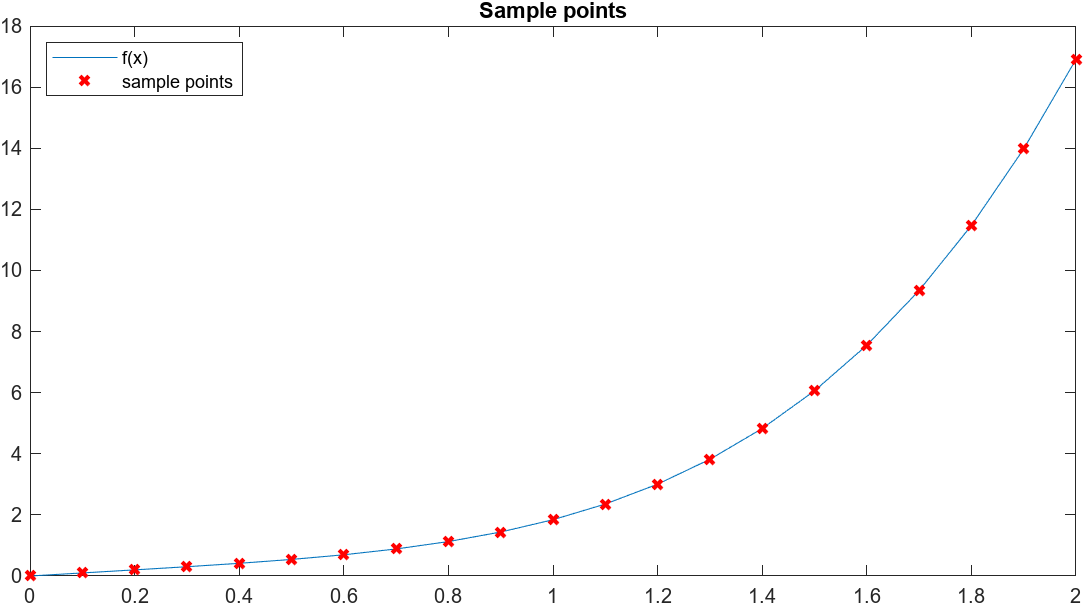
\includegraphics[width=0.8\columnwidth]{img/sample_points.png} 
	\caption{Sample Points of f(x)}
	\label{fig:sample_points}
\end{figure}

After applying second-order accurate difference approximations, I draw $f'(x)$ and $f''(x)$ to check the difference between a real derivative and finite difference schemes.

\begin{figure}[h!]
	\centering
	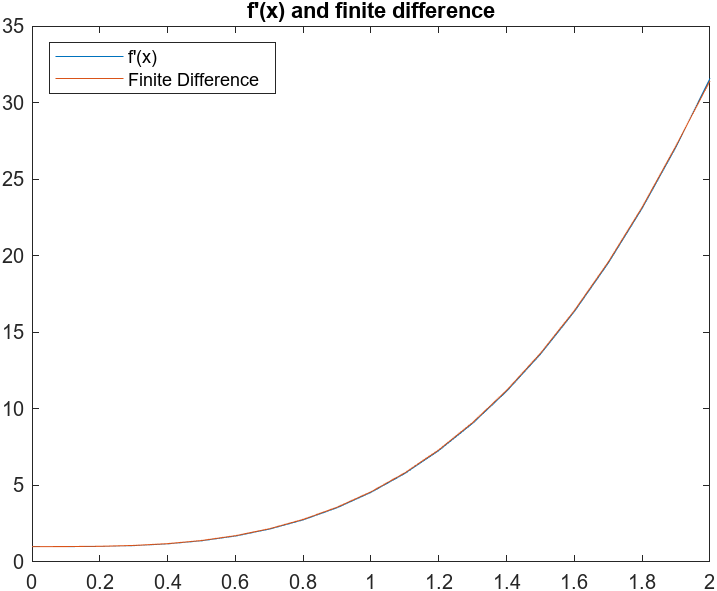
\includegraphics[width=0.8\columnwidth]{img/f'(x).png} 
	\caption{Compare real first derivative and finite difference}
	\label{fig:f'(x)}
\end{figure}

\begin{figure}[h!]
	\centering
	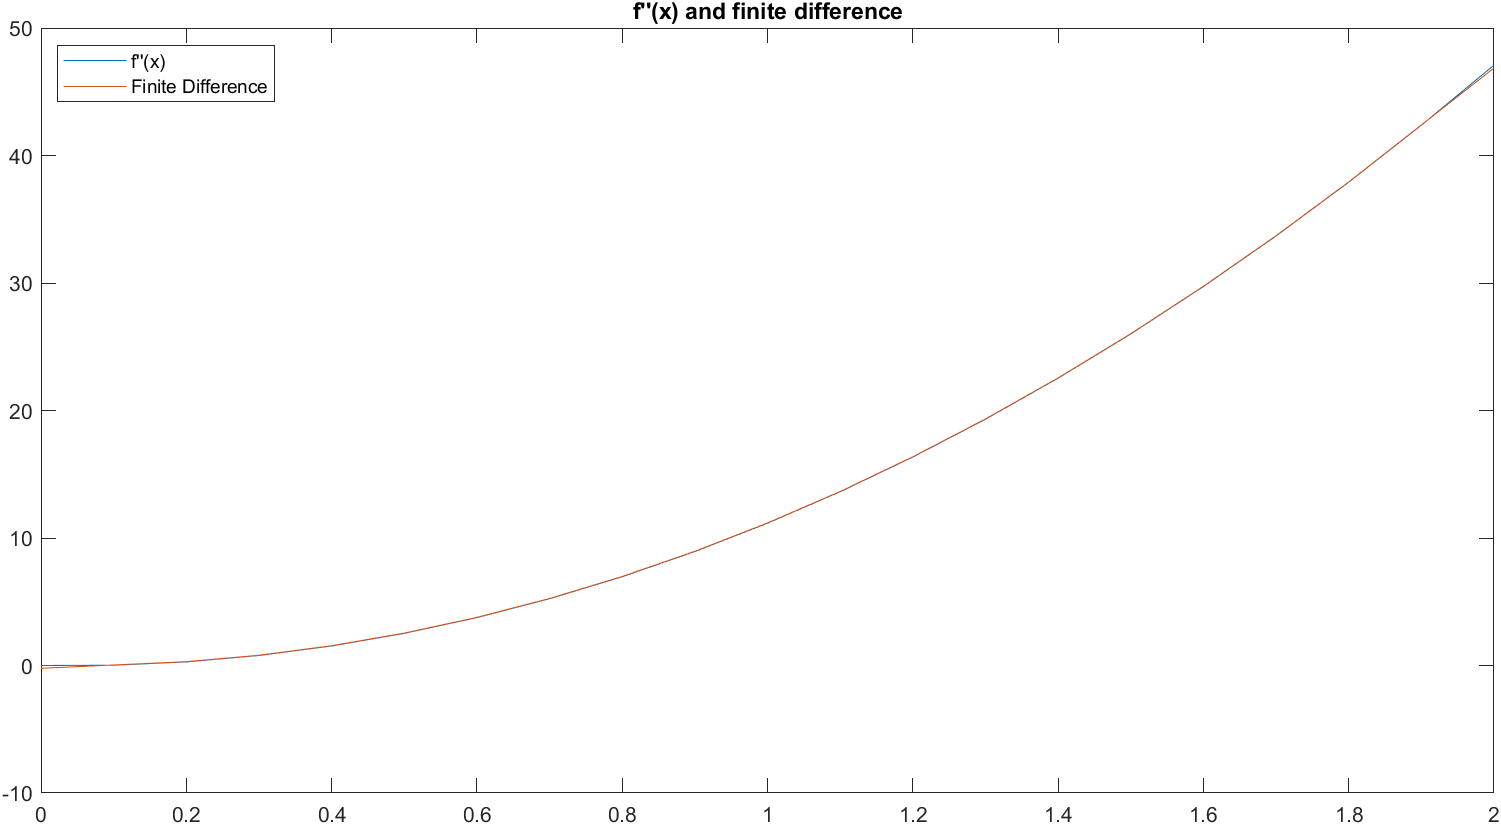
\includegraphics[width=0.8\columnwidth]{img/f''(x).png} 
	\caption{Compare real second derivative and finite difference}
	\label{fig:f''(x)}
\end{figure}


Figure.\ref{fig:f'(x)} and Figure.\ref{fig:f''(x)} told us that the second-order accurate difference approximations are close to the real derivative, even their actual difference. 
And I compared the deviations of the difference approximations with the actual difference.
It can be found that both the first-order derivatives Figure.\ref{fig:error_f'(x)} and the second-order \ref{fig:error_f''(x)} derivatives are better than the forward and backward differential approximations, which is why we need to use the central differential approximation as much as possible and only use the forward and backward differential approximations at the endpoints.
You can find more implementation detail in the code.

\begin{figure}[h!]
	\centering
	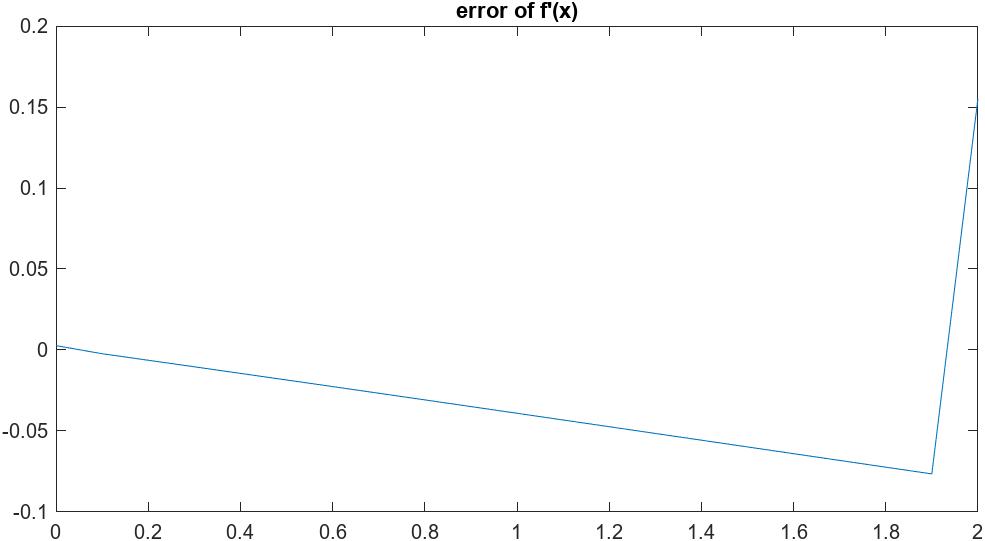
\includegraphics[width=0.8\columnwidth]{img/error_f'(x).png} 
	\caption{errors of f'(x)}
	\label{fig:error_f'(x)}
\end{figure}

\begin{figure}[h!]
	\centering
	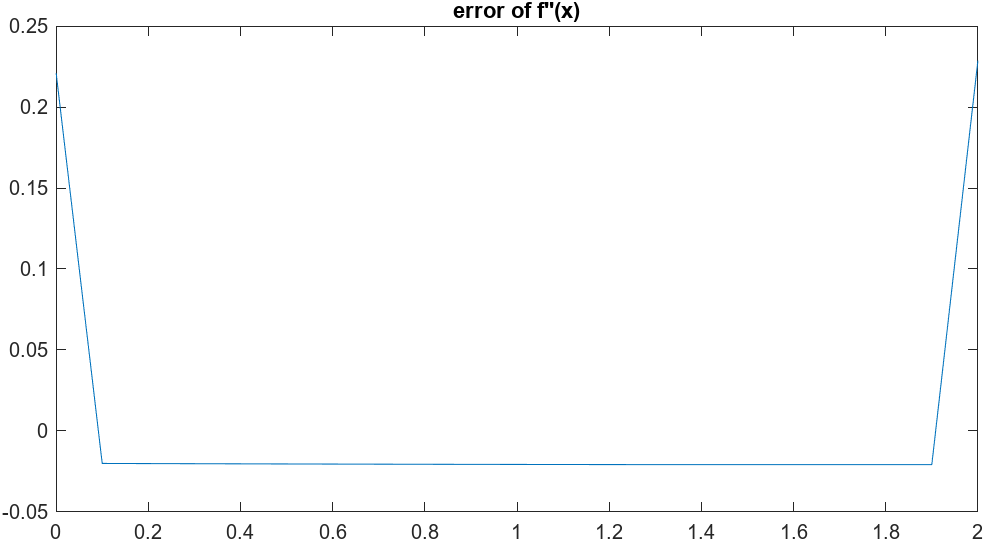
\includegraphics[width=0.8\columnwidth]{img/error_f''(x).png} 
	\caption{errors of f''(x)}
	\label{fig:error_f''(x)}
\end{figure}

%----------------------------------------------------------------------------------------

\section{Topic 2}

\subsection*{Answer}

To evaluate double integrals which are performed on the rectangle $R = \{ (x, y) \in \mathbb{R}^2: a \leq x \leq b \text{ and } c \leq y \leq d  \} $, We first consider the uniform-grid in each
dimension. Let grid space of $x$ and $y$ be the $h$, which means we have $x_1, x_2, \ldots , x_{n_x}$ and $y_1, y_2, \ldots , y_{n_y}$.\cite{numinteg} \cite{nume}
For integrals in one dimension, we could start with something simple like the trapezoidal rule

\begin{equation}
	\int^{b}_{a}f(x)dx\approx \frac{h}{2}[f(a) + f(b) + 2\sum^{n-1}_{i=2}f(x_i)]
\end{equation}

We can now extend this definition to the two-dimensional case, i.e

\begin{equation}
	A_{2D}=\int^{c}_{d}\int^{a}_{b}f(x, y)\, dxdy = \int^{c}_{d}g(y)\, dy
\end{equation}

where, 
\begin{equation}
	g(y) = \int^{b}_{a}f(x,y)\,dx 
\end{equation}

\subparagraph*{Task 1}
Now apply the trapezoidal rule to calculate the integral to $x$ with fixed $y$.
\begin{equation} \label{g(y)}
	\begin{aligned}
		g(y) & = \int^{b}_{a}f(x,y)\,dx                                                 \\
		     & = \sum^{n_x-1}_{i=1}\frac{1}{2}[f(x_i)+f(x_{i+1})]h                      \\
		     & = \frac{h}{2} [f(x_0, y) + f(x_{n_x}, y) + 2\sum^{n_x-1}_{i=2}f(x_i, y)] \\
		     & = \frac{h}{2} [f(a, y) + f(b, y) + 2\sum^{n_x-1}_{i=2}f(x_i, y)]
	\end{aligned}
\end{equation}

Finally we get $g(y)=\frac{h}{2} [f(a, y) + f(b, y) + 2\sum^{n_x-1}_{i=2}f(x_i, y)]$

\subparagraph*{Task 2}
After integrate $x$, we now integrate $y$,
\begin{equation} \label{I}
	\begin{aligned}
		I & = \int^{d}_{c}g(y)\,dy                                  \\
		%   &= \int^{d}_{c}\frac{h}{2} [f(a, y) + f(b, y) + 2\sum^{n_x-1}_{i=2}f(x_i, y)] \,dy \\
		  & = \sum^{n_y-1}_{i=1}\frac{1}{2} [g(y_i)+g(y_{i+1})]h    \\
		  & = \frac{h}{2} [g(c) + g(d) + 2\sum^{n_y-1}_{j=2}g(y_j)]
	\end{aligned}
\end{equation}
Substituting eq.\eqref{g(y)} into  eq.\eqref{I} we have
\begin{equation}
	\begin{aligned} \label{substitutedI}
		I = \frac{h}{2}\{ & \frac{h}{2}[f(a, c) + f(b, c) + 2\sum^{n_x-1}_{i=2}f(x_i, c)]                            \\
		+                 & \frac{h}{2}[f(a, d) + f(b, d) + 2\sum^{n_x-1}_{i=2}f(x_i, d)]                            \\
		+                 & \frac{h}{2}2\sum^{n_y-1}_{j=2}[f(a, y_j) + f(b, y_j) + 2\sum^{n_x-1}_{i=2}f(x_i, y_j)]\}
	\end{aligned}
\end{equation}

Now we can simplify eq.\eqref{substitutedI} as much as possible
\begin{equation}
	\begin{aligned}
		I = (\frac{h}{2})^2[ & f(a, c)+f(b, c)+f(a, d)+f(b, d)                   \\
		+                    & 2\sum^{n_x-1}_{i=2}[f(x_i, c)+f(x_i, d)]          \\
		+                    & 2\sum^{n_y-1}_{j=2}[f(a, y_j)+f(b, y_j)]          \\
		+                    & 4\sum^{n_y-1}_{j=2}\sum^{n_x-1}_{i=2}f(x_i, y_j)]
	\end{aligned}
\end{equation}


\subsection*{Implement}

Here is the implemented code with Matlab. 
I used a for-loop to implement the above algorithm. $my\_integral2$ function takes 5 parameters: 
\begin{enumerate}[itemindent=1em, label=•]
	\item \textbf{f}: the function
	\item \textbf{a, b}: the start and end points of x, 
	\item \textbf{c, d}: the start and end points of y, 
	\item \textbf{h}: the length of the partition (for comparing computational accuracy)
\end{enumerate}
For the four summation symbols in the formula, I use four for-loops to traverse all the elements and sum them and then get the integral result.

\begin{lstlisting}
	function I=my_integral2(f, a, b, c, d, h)
		x=a:h:b;
		y=c:h:d;

		n_x=length(x);
		n_y=length(y);
		I=f(a, c)+f(b,c)+f(a,d)+f(b,d);


		for i=2:n_x-1
			I = I + 2*(f(x(i),c)+f(x(i),d));
		end


		for j=2:n_y-1
			I = I + 2*(f(a, y(j))+f(b, y(j)));
		end

		
		for i=2:n_x-1
			for j=2:n_y-1
				I = I + 4*f(x(i), y(j));
			end
		end

		I = h^2/4*I;
	end
\end{lstlisting}

After doing some experiments, I found that the finer the segmentation and the larger the rectangle, the higher the accuracy can be obtained. You can see more detailed data in the following two tables (Table \ref{table1}) (Table \ref{table2}).
Here I use the formula $\frac{\left\lvert my\_integral2-real\right\rvert }{\left\lvert real\right\rvert }$ to calculate the error.

\begin{table*}
	\centering
	\caption{Accuracy of difference h with function $y^4+\sin(x)$}
	\label{table1}
	\begin{tabular}{ccc}
		\toprule
		               & a=0;b=1;c=2;d=4;h=0.1 & a=0;b=1;c=2;d=4;h=0.5 \\
		\midrule
		my\_integral2  & 199.505289            & 203.962661            \\
		real           & 199.319395            & 199.319395            \\
		\textbf{error} & \textbf{0.0933\%}     & \textbf{2.3296\%}     \\
		\bottomrule
	\end{tabular}
\end{table*}

\begin{table*}
	\centering
	\caption{Accuracy of difference R with function $y^4+\sin(x)$}
	\label{table2}
	\begin{tabular}{ccc}
		\toprule
		               & a=0;b=1;c=2;d=4;h=0.1 & a=0;b=1;c=0;d=10;h=0.1 \\
		\midrule
		my\_integral2  & 199.505289            & 20007.926445           \\
		real           & 199.319395            & 20004.596977           \\
		\textbf{error} & \textbf{0.0933\%}     & \textbf{0.0166\%}      \\
		\bottomrule
	\end{tabular}
\end{table*}
\clearpage
\newpage
\bibliographystyle{plain}
\bibliography{ref.bib} 
\end{document}